\documentclass[fleqn, a4paper, 12pt]{amsart}
\usepackage{amsmath, amssymb, amsthm}
%\usepackage{gensymb}
\usepackage{commath}
\usepackage{xcolor}
\usepackage{cancel}
\usepackage{siunitx}
\usepackage{tikz, pgfplots}
\usetikzlibrary{calc, hobby, patterns}
\usepackage{graphicx}
\usepackage{hyperref}
\usepackage{datetime}
\usepackage{ulem}
\usepackage{xfrac}
\usepackage{asymptote}
\usepackage{enumerate}
\setcounter{secnumdepth}{4}
\newcommand\numberthis{\addtocounter{equation}{1}\tag{\theequation}}

\newcommand{\AxisRotator}[1][rotate=0]{%
	\tikz [x=0.25cm,y=0.60cm,line width=.2ex,-stealth,#1] \draw (0,0) arc (-150:150:1 and 1);%
}

\theoremstyle{definition}
\newtheorem{example}{Example}
\newtheorem{definition}{Definition}

\theoremstyle{theorem}
\newtheorem{theorem}{Theorem}

\newenvironment{solution}
{\begin{proof}[Solution]\let\qed\relax}
	{\end{proof}}

\newcommand{\curl}{\mathrm{curl\,}}

%\renewcommand{\int_{min}^{max}}{\int\displaylimits_{min}^{max}}

%opening
\title{Lecture 14}
\author{Aakash Jog}
\date{\formatdate{16}{12}{2014}}

\begin{document}

\maketitle
%\setlength{\mathindent}{0pt}

\tableofcontents

\newpage
\section{Rigid Body Mechanics}

\subsection{Definitions}
\hspace{1cm}\\
\begin{figure}[h]
	\begin{tikzpicture}
		\coordinate (O) at (0, 0);
		
		\def\l{4};
		
		\coordinate (rod top) at (0, {\l/2});
		\coordinate (rod bottom) at (0, {-\l/2});
		
		\fill [red] (O) circle [radius = 1pt];
		
		\draw [ultra thick] (rod bottom) -- (rod top);
		
		\draw [stealth-] (O) -- ++(1,0) node [right] {$F$};
		\draw [stealth-] (O) -- ++(-1,0) node [left] {$F$};
	\end{tikzpicture}
\end{figure}

\begin{align*}
	M_{\text{total}} \overrightarrow{a_{\text{COM}}} &= \sum \overrightarrow{F_{\text{ext}}}\\
	\therefore v_{\text{COM}} &= \text{ constant }
\end{align*}

\begin{figure}[h]
	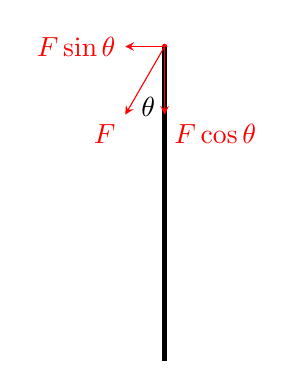
\begin{tikzpicture}
		\coordinate (O) at (0, 0);
		
		\def\l{4};
		\def\angle{30}
		
		\coordinate (rod top) at (0, 0);
		\coordinate (rod bottom) at (0, -\l);
		
		\fill [red] (O) circle [radius = 1pt];
		
		\draw [ultra thick] (rod bottom) -- (rod top);
		
		\node at ({270-\angle/2}:0.8) {$\theta$};
		
		\draw [-stealth, red] (rod top) -- ++({270-\angle}:1) node [below left] {$F$};
		\draw [-stealth, red] (rod top) -- ++({180}:{1*sin(\angle)}) node [left] {$F \sin \theta$};
		\draw [-stealth, red] (rod top) -- ++({270}:{1*cos(\angle)}) node [below right] {$F \cos \theta$};
	\end{tikzpicture}
\end{figure}

\begin{definition}[Torque]
	\begin{align*}
		\tau &\doteq r F \sin \theta\\
		\overrightarrow{\tau} &\doteq \overrightarrow{r} \times \overrightarrow{F}
	\end{align*}
\end{definition}

\begin{definition}[Angular momentum]
	\begin{align*}
		\overrightarrow{L} &\doteq \overrightarrow{r} \times \overrightarrow{p}
	\end{align*}
\end{definition}

\begin{align*}
	\overrightarrow{\tau_A} &= 0\\
	\therefore \dod{\overrightarrow{L_A}}{t} &= 0\\
	\therefore \overrightarrow{L_A} &= \text{ constant }\\
	&= r m v \hat{z}\\
	&= m r^2 \omega \hat{z}\\
	&= (m r^2) \overrightarrow{\omega}
\end{align*}

\begin{definition}[Moment of Inertia]
	\begin{align*}
		I &\doteq m r^2
	\end{align*}
\end{definition}

\begin{align*}
	E_k &= \dfrac{1}{2} m v^2\\
	&= \dfrac{1}{2} m r^2 \omega^2\\
	&= \dfrac{1}{2} I \omega^2
\end{align*}

\begin{example}
	A particle attached to a string is on a horizontal table, moving in a circle of radius $r_0$ with $v_0$. The other end on the string goes through the table, through a hole in the centre of the circle. It is pulled down by a force $F$. Find the velocity of the particle as a function of the radius.
\end{example}

\begin{solution}
	\begin{align*}
		\overrightarrow{\tau} &= 0\\
		\therefore \overrightarrow{L_A} &= r_0 m v_0 \hat{z}\\
		\therefore \overrightarrow{L} &= r m v \hat{z}
	\end{align*}
\end{solution}

\begin{example}
	\begin{figure}[h]
		\begin{tikzpicture}
			\coordinate (O) at (0,0);
			
			\coordinate (m1) at (5*rnd, 5*rnd);
			\coordinate (m2) at (-4*rnd, 4*rnd);
			
			\fill (m1) circle [radius = 1pt] node [right] {$m_1$};
			\fill (m2) circle [radius = 1pt] node [left] {$m_2$};
			
			\fill (O) circle [radius = 0.8pt] node [below] {$O$};
			
			\draw [-stealth] (O) -- (m1) node [midway, fill = white] {$\overrightarrow{r_1}$};
			\draw [-stealth] (O) -- (m2) node [midway, fill = white] {$\overrightarrow{r_2}$};
			
			\draw [-stealth, red] (m1) -- ++(rnd, rnd) node [above] {$\overrightarrow{F_{1, \text{ ext }}}$};
			\draw [-stealth, red] (m2) -- ++(rnd, rnd) node [above] {$\overrightarrow{F_{1, \text{ ext }}}$};
			
		\end{tikzpicture}
	\end{figure}
\end{example}

\begin{solution}
	\begin{align*}
		\overrightarrow{F_{1,2}} &= - \overrightarrow{F_{2,1}}\\
		\overrightarrow{\tau_{\text{ total }, 0}} &= \overrightarrow{\tau_{1, 0}} + \overrightarrow{\tau_{2, 0}}\\
		&= \overrightarrow{r_1} \times \overrightarrow{F_{1, \text{ ext }}} + \overrightarrow{r_1} \times \overrightarrow{F_{1, 2}} + \overrightarrow{r_2} \times \overrightarrow{F_{2, \text{ ext }}} + \overrightarrow{r_2} \times \overrightarrow{F_{2, 1}}\\
		&= \overrightarrow{r_1} \times \overrightarrow{F_{1, \text{ ext }}} + \overrightarrow{r_2} \times \overrightarrow{F_{2, \text{ ext }}} + \cancelto{0}{(\overrightarrow{r_1} - \overrightarrow{r_2}) \times \overrightarrow{F_{1, 2}}}\\
		&= \overrightarrow{\tau_{\text{ total}, O, {\text{ ext }}}}
	\end{align*}
\end{solution}

\subsection{Conditions for Equilibrium}

\begin{figure}[h]
	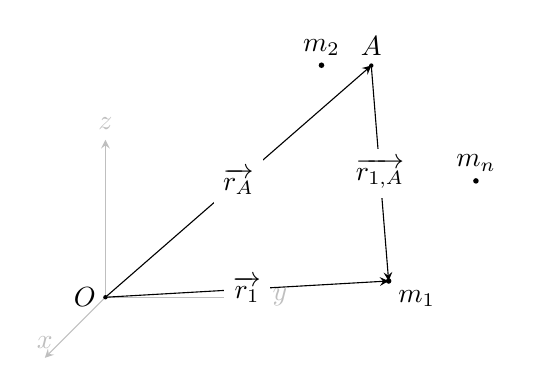
\begin{tikzpicture}
		%definition of origin
		\coordinate (O) at (0,0,0); 
		
		%definition of minimum and maximum values for axes
		\def\xMIN{0};
		\def\yMIN{0};
		\def\zMIN{0};
		\def\xMAX{2};
		\def\yMAX{2};
		\def\zMAX{2};
		
		%axes
		\draw [-stealth, lightgray] (\xMIN,0,0) -- (\xMAX,0,0) node [right] {$y$}; 
		\draw [-stealth, lightgray] (0,\yMIN,0) -- (0,\yMAX,0) node [above] {$z$};
		\draw [-stealth, lightgray] (0,0,\zMIN) -- (0,0,\zMAX) node [above] {$x$};
		
		\fill (O) circle [radius = 0.8pt] node [left] {$O$};
		
		%point masses
		\coordinate (m1) at (4+rnd, 1+rnd, 3+rnd);
		\coordinate (m2) at (2+rnd, 3+rnd, rnd);
		\coordinate (mn) at (5+rnd, 2+rnd, 2+rnd);
		
		\fill (m1) circle [radius = 1pt] node [below right] {$m_1$};
		\fill (m2) circle [radius = 1pt] node [above] {$m_2$};
		\fill (mn) circle [radius = 1pt] node [above] {$m_n$};
		
		\draw [-stealth] (O) -- (m1) node [midway, fill = white] {$\overrightarrow{r_1}$};
		
		%alternate origin
		\coordinate (A) at (5+rnd, 5+rnd, 5+rnd);
		
		\fill (A) circle [radius = 0.8pt] node [above] {$A$};
		
		\draw [-stealth] (O) -- (A) node [midway, fill = white] {$\overrightarrow{r_A}$};
		
		\draw [-stealth] (A) -- (m1) node [midway, fill = white] {$\overrightarrow{r_{1, A}}$};
	\end{tikzpicture}
\end{figure}

\begin{align*}
	\sum \overrightarrow{F_{i, \text{ ext }}} &= 0\\
	\sum \overrightarrow{\tau_{i, O, \text{ ext }}} &= 0
\end{align*}

\begin{align*}
	\sum \overrightarrow{\tau_{i, A, \text{ ext }}} &= \sum \overrightarrow{r_{i, A}} \times \overrightarrow{F_{i, \text{ ext }}}\\
	&= \sum \overrightarrow{r_{i, O}} \times \overrightarrow{F_{i, \text{ ext }}} - \sum \overrightarrow{r_A} \times \overrightarrow{F_{i, \text{ ext }}}\\
	&= 0
\end{align*}
Therefore, equilibrium is independent of the point of reference.\\
Hence the conditions for equilibrium are
\begin{align*}
	\sum \overrightarrow{F_{i, \text{ ext }}} &= 0\\
	\sum \overrightarrow{\tau_{i, \text{ ext }}} &= 0
\end{align*}

\begin{example}
	Find the minimum $\mu$ for which the bodies remain at rest.
	\begin{figure}[h]
		\begin{tikzpicture}[scale=0.5]
			\coordinate (O) at (0,0);
			
			\def\r{3};
			\def\xMIN{-3*\r};
			\def\xMAX{3*\r};
						
			\coordinate (c1) at (\r,\r);
			\coordinate (c2) at (-\r,\r);
			\coordinate (c3) at ($(c2)+(60:2*\r)$);
			
			\draw (\xMIN, 0) -- (\xMAX, 0);
			
			\draw (c1) circle [radius = \r];
			\draw (c2) circle [radius = \r];
			\draw (c3) circle [radius = \r];
			
			%forces on disk 1
			\draw [-stealth, red] (c1) -- ++(-90:1) node [right] {$mg$};
			\draw [-stealth, red] (c1)++(-90:\r) -- ++(90:1) node [right] {$mg$};
		\end{tikzpicture}
	\end{figure}
\end{example}

\begin{solution}
	\begin{align*}
		\sum \overrightarrow{F_{i, \text{ ext }}} &= 0\\
		\therefore 2 N_f &= 3 m g\\
		\therefore N_f &= \dfrac{3}{2} m g
	\end{align*}
	With respect to an axis passing through $A$,
	\begin{align*}
		\sum \overrightarrow{\tau_{i, \text{ ext }}} &= 0\\
		\therefore (-\hat{z}) d m g + \hat{z} d \cdot \dfrac{3}{2} m g + (-\hat{z}) H f_f &= 0\\
		\therefore f_f &= \dfrac{\sfrac{1}{2} \cdot m g d}{H}\\
		&= \dfrac{\sfrac{1}{2} \cdot m g R \cos 60}{R + R \sin 60}\\
		&\leq \mu N_f\\
		\therefore \dfrac{\sfrac{1}{2} \cdot m g \cdot \sfrac{1}{2}}{1 + \sfrac{\sqrt{3}}{2}} &= \mu \cdot \sfrac{3}{2} \cdot m g\\
		\therefore \mu &\geq \dfrac{\sfrac{1}{6}}{1 + \sfrac{\sqrt{3}}{2}}
	\end{align*}
\end{solution}

\section{Coordinate Systems}

\subsection{Cylindrical Coordinates}

\begin{align*}
	(x, y, z) &\to (r, \theta, z)
\end{align*}
\begin{align*}
	x &= r \cos \theta\\
	y &= r \sin \theta\\
	z &= z
\end{align*}

\begin{figure}[h]
	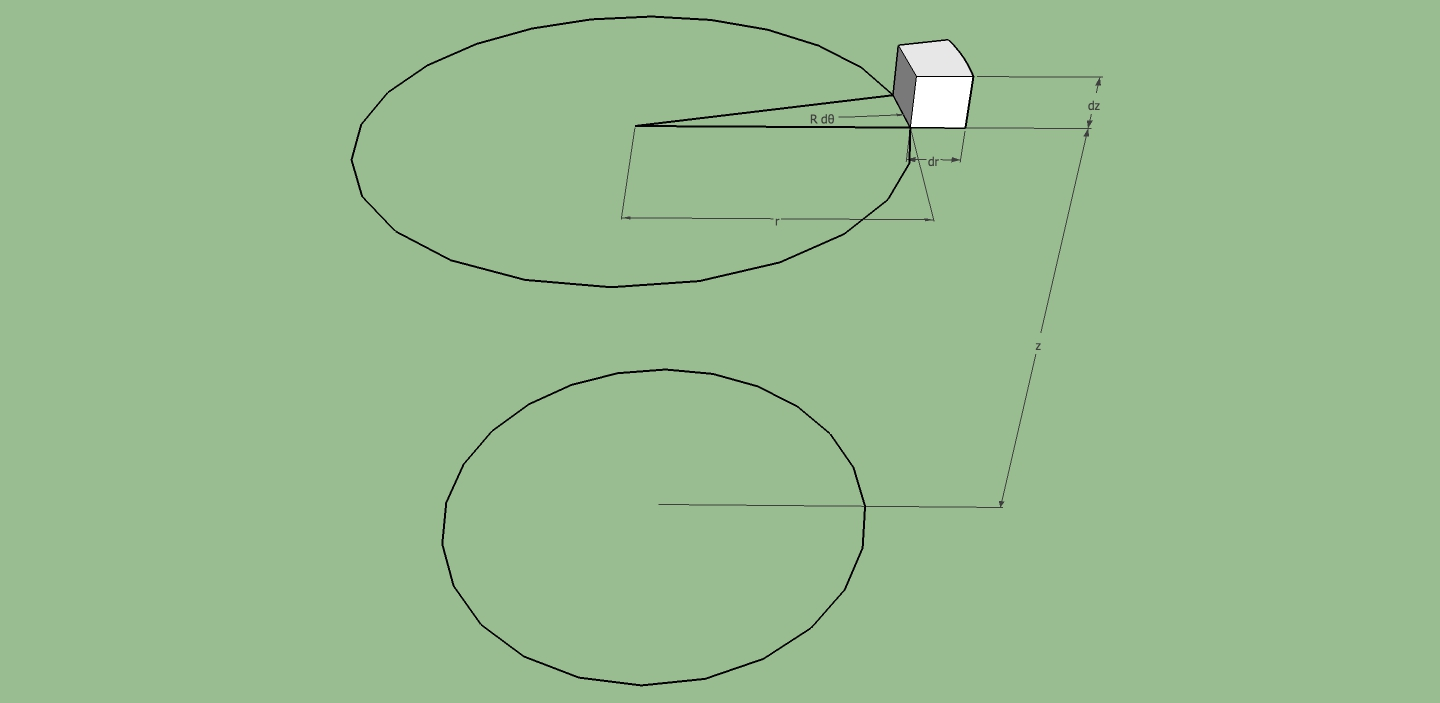
\includegraphics[width=\textwidth]{CylindricalCoordinates.jpg}
\end{figure}

\begin{align*}
	\dif V &= r \dif \theta \dif r \dif z
\end{align*}

\subsection{Spherical Coordinates}

\begin{align*}
(x, y, z) &\to (r, \theta, \varphi)
\end{align*}

\begin{figure}[h]
	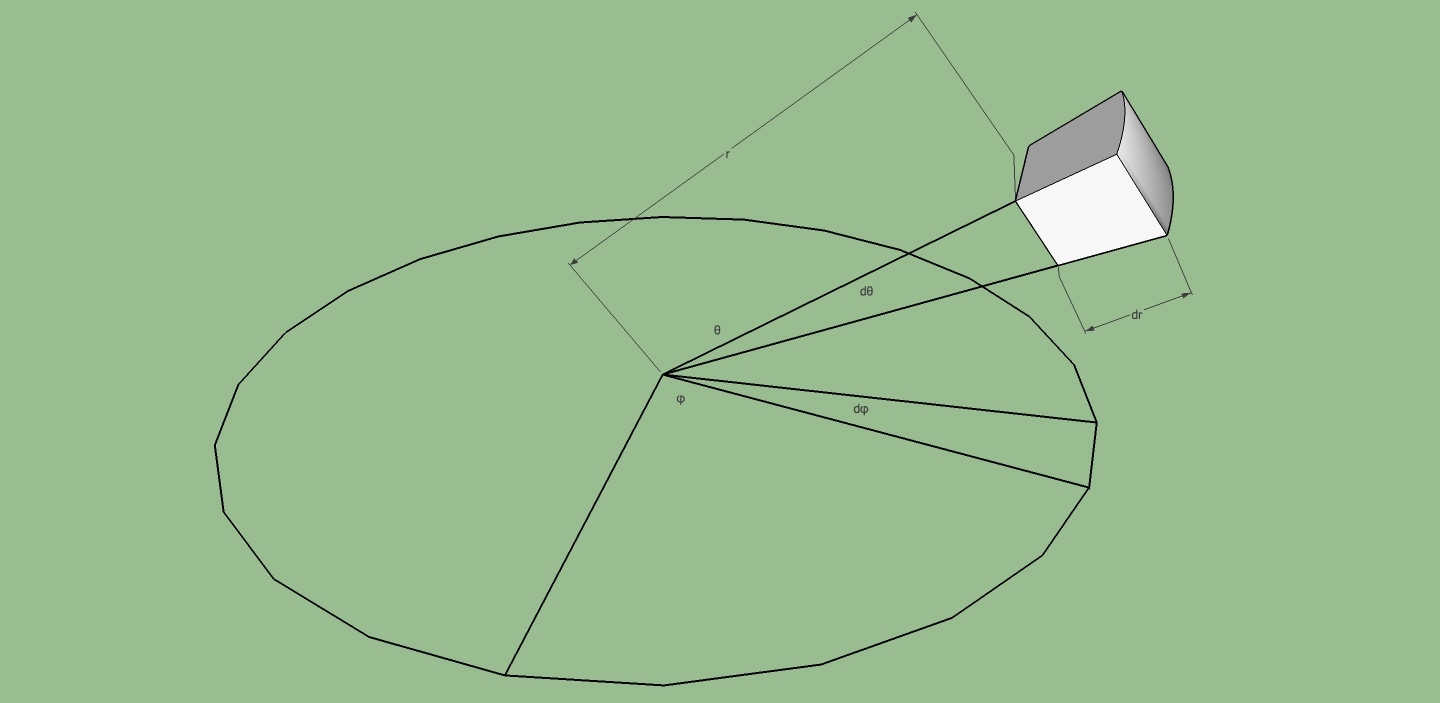
\includegraphics[width=\textwidth]{SphericalCoordinates.jpg}
\end{figure}

\begin{align*}
	\dif V &= r \dif \theta \cdot r \sin \theta \dif \varphi \dif r\\
	&= r^2 \sin \theta \dif \varphi \dif r \dif \theta
\end{align*}

\end{document}